\null
\begin{tikzpicture}[remember picture, overlay]

  % 1. Cụm 4 đường kẻ cyan ở lề trên bên trái
  \draw[stewartcyan, line width=1.2pt] ([xshift=0pt, yshift=-66pt]current page.north west) -- ([xshift=42pt, yshift=-66pt]current page.north west);
  \draw[stewartcyan, line width=1.2pt] ([xshift=0pt, yshift=-71pt]current page.north west) -- ([xshift=42pt, yshift=-71pt]current page.north west);
  \draw[stewartcyan, line width=1.2pt] ([xshift=0pt, yshift=-76pt]current page.north west) -- ([xshift=42pt, yshift=-76pt]current page.north west);
  \draw[stewartcyan, line width=1.2pt] ([xshift=0pt, yshift=-81pt]current page.north west) -- ([xshift=42pt, yshift=-81pt]current page.north west);

  % 2. Ảnh đầu chương (Cliff Diver) tràn viền trên và phải
  \node[anchor=north east, inner sep=0pt] at ([xshift=612pt, yshift=0pt]current page.north west) {%
    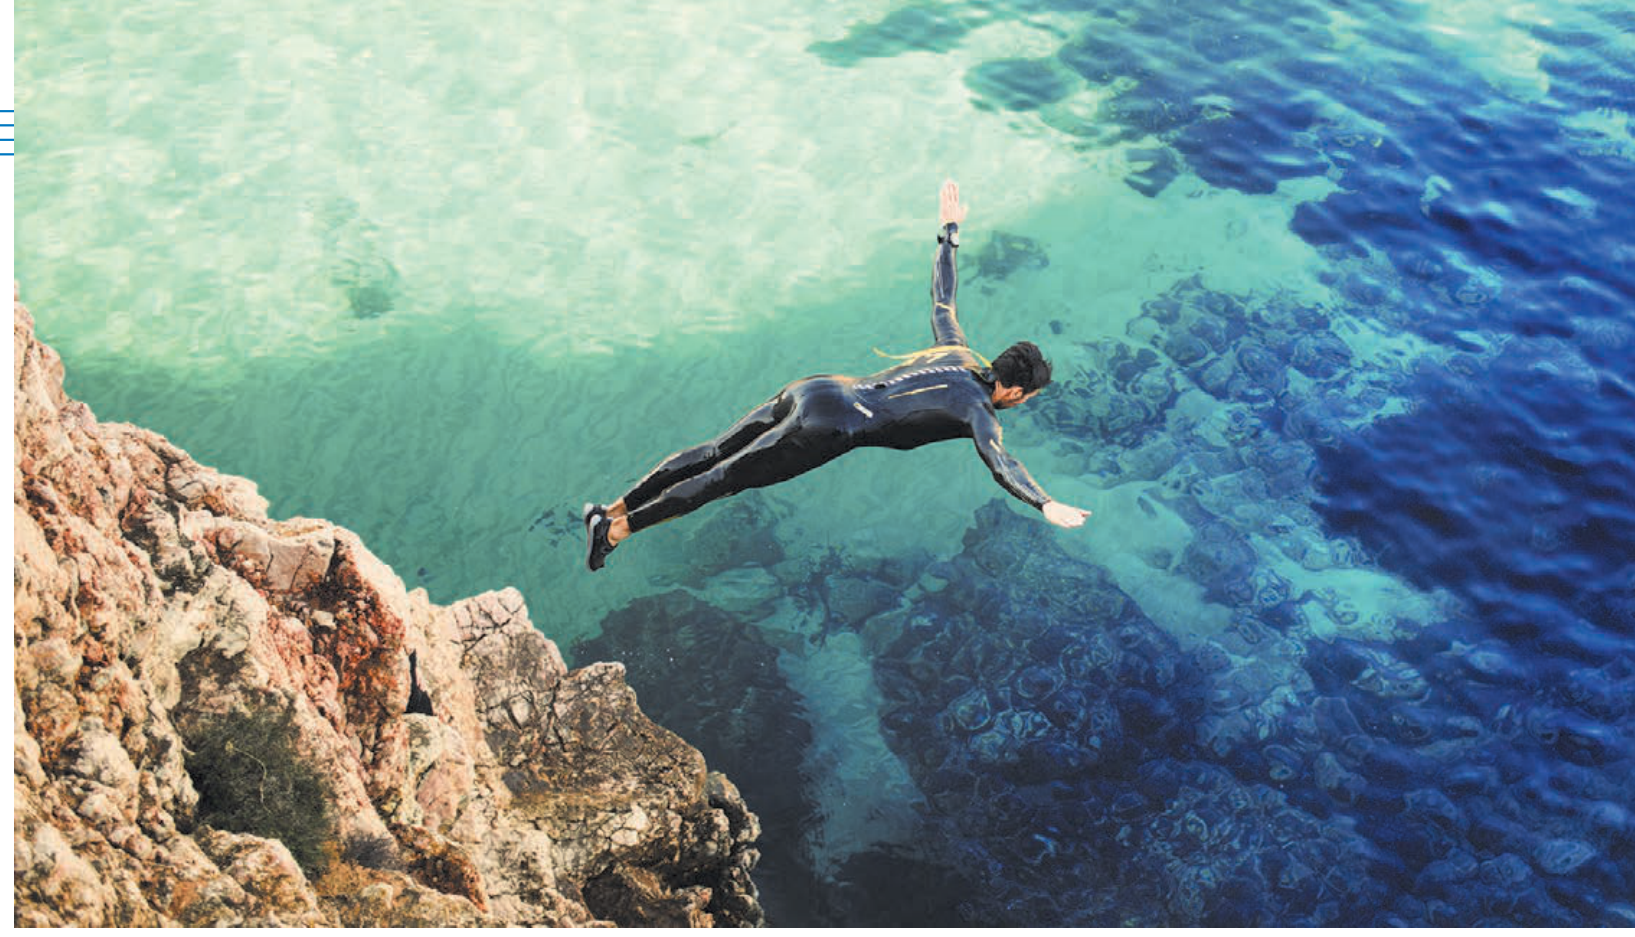
\includegraphics[width=570pt, height=292pt]{images/p0112_fig1.png}%
  };

  % 3. Chú thích hình ảnh & bản quyền ở cột lề trái bên dưới ảnh
  \node[anchor=north west, inner sep=0pt] at ([xshift=42pt, yshift=-310pt]current page.north west) {%
    \begin{minipage}{295pt}
      {\fontsize{8.5}{11.5}\selectfont\sffamily\bfseries\color{stewartdark}%
      Chúng ta biết rằng khi một vật rơi từ trên cao xuống, nó sẽ rơi ngày càng nhanh hơn. Galileo đã phát hiện ra rằng quãng đường mà vật rơi được tỉ lệ thuận với bình phương thời gian trôi qua. Giải tích cho phép chúng ta tính toán vận tốc chính xác của vật tại bất kỳ thời điểm nào. Trong Bài tập 2.7.11, bạn sẽ được yêu cầu xác định vận tốc mà tại đó một người nhảy vách đá lao mình xuống đại dương.\par}
      \vspace{3pt}
      {\fontsize{7}{9}\selectfont\sffamily\color{creditgray}Icealex / Shutterstock.com\par}
    \end{minipage}%
  };

  % 4. Đường kẻ dọc cyan phân cách cột lề và nội dung chính
  \draw[stewartcyan, line width=1.5pt] ([xshift=112pt, yshift=-356pt]current page.north west) -- ([xshift=112pt, yshift=-705pt]current page.north west);

  % 5. Số thứ tự chương "2"
  \node[anchor=north east, inner sep=0pt] at ([xshift=100pt, yshift=-365pt]current page.north west) {%
    {\fontsize{74}{74}\selectfont\sffamily\bfseries\color{stewartcyan}2}%
  };

  % 6. Tiêu đề chương "Giới hạn và Đạo hàm"
  \node[anchor=north west, inner sep=0pt] at ([xshift=126pt, yshift=-372pt]current page.north west) {%
    {\fontsize{28}{34}\selectfont\sffamily\bfseries\color{stewartdark}Giới hạn và Đạo hàm}%
  };

  % 7. Đoạn văn dẫn nhập chương
  \node[anchor=north west, inner sep=0pt] at ([xshift=126pt, yshift=-440pt]current page.north west) {%
    \begin{minipage}{435pt}
      \fontsize{10}{14.2}\selectfont\rmfamily\color{stewartdark}%
      \noindent{\sffamily\bfseries TRONG PHẦN TỔNG QUAN VỀ GIẢI TÍCH} (ngay trước Chương 1), chúng ta đã thấy ý tưởng về giới hạn làm nền tảng cho các nhánh khác nhau của giải tích như thế nào. Do đó, việc bắt đầu nghiên cứu giải tích bằng cách khảo sát các giới hạn và tính chất của chúng là hoàn toàn phù hợp. Dạng giới hạn đặc biệt được sử dụng để tìm tiếp tuyến và vận tốc đã làm nảy sinh ý tưởng trọng tâm trong phép tính vi phân: đạo hàm.
    \end{minipage}%
  };

  % 8. Số trang 77 ở góc dưới bên phải
  \node[anchor=base east, inner sep=0pt] at ([xshift=561pt, yshift=-678pt]current page.north west) {%
    {\fontsize{11}{11}\selectfont\sffamily\bfseries\color{stewartdark}77}%
  };

\end{tikzpicture}
